\section{Maze-Khepera data (class)}
\label{sec:mkd}

\subsection{Introduction}
\label{sec:mkd:intro}

From the detector, we have a discrete description of the maze, but it 
is still unreadable for the maze plant. To make use if it, I wrapped 
the MazeData class that defines the maze structure used by the maze 
plant. The wrapper takes in parameter the Tapirdetector, reads the blocks 
from the detector and writes a maze definition file that MazaData 
can read.

\subsection{Convert detector information to maze data}
\label{sec:mkd:algo}
Here is the algorithm described in chronological order.

\marginpar{
        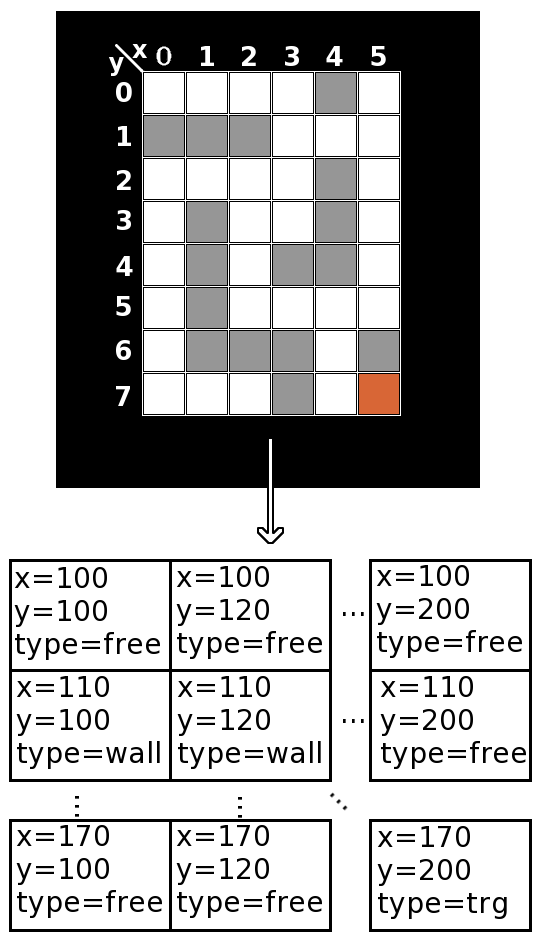
\includegraphics[width=4.5cm]{./img/MazeKheperaData.png}
        \captionof{figure}[Structure of the list of detected objects]{%
        Structure of the list of detected objects --
        Each block of the grid is represented as a blob with 
        the attributes $x$, $y$ and $type$ which are mapped to the 
        attributes $x$, $y$, $size$ of the opencv blob object.
        $x$ and $y$ are left-upper values on the image, noted as $x_i$, 
        $y_i$, not to confuse with the grid values $x_g$, $y_g$. The objects
        are listed from left to right, from top to bottom.}
        \label{fig:mkd:struct}
    }


    \begin{enumerate}
        \item It first get the maze description from TapirDetector.
        \item It calculates the maze boundaries ($x_{min}$, $x_{max}$, 
            $y_{min}$, $y_{max}$, $x_{extend}$ and $y_{extend}$):
        \begin{enumerate}
            \item Min and max are calculated regarding minimum and maximum 
                positions of the blocks. (Do not forget that the detector 
                can detect a subframe of the image, thus min and max 
                values are important)
            \item Since we have upper-left position of the blocks (see
                point \ref{sec:cgd:algo:blockattributs}. of 
                section \ref{sec:cgd:algo}), 
                $x_{min}$ and $y_{min}$ correspond to exact $x_{min}$ 
                and $y_{min}$ values 
                but $\tilde{x}_{max}$ and $\tilde{y}_{max}$ are the upper-left position of the 
                max block. Thus, real $x_{max}$ and $y_{max}$ are 
                $\tilde{x}_{max}+gridwidth_x$ and 
                $\tilde{y}_{max}+gridwidth_y$.
            \item $x_{extend}$, $y_{extend}$ = $grid_x$, $grid_y$ 
                (number of different 
                $x$ and $y$ positions)
        \end{enumerate}
        \item It builds a grid to save the maze info.
        \item It loops through the blocks and save the type information
            in the grid.
        \item Once the grid is build, it saves it in a file as a maze
            definition. 
        \item MazeData is constructed using the saved file maze.
    \end{enumerate}

\subsection{Improvements}
\label{sec:mkd:improvements}

\marginpar{
        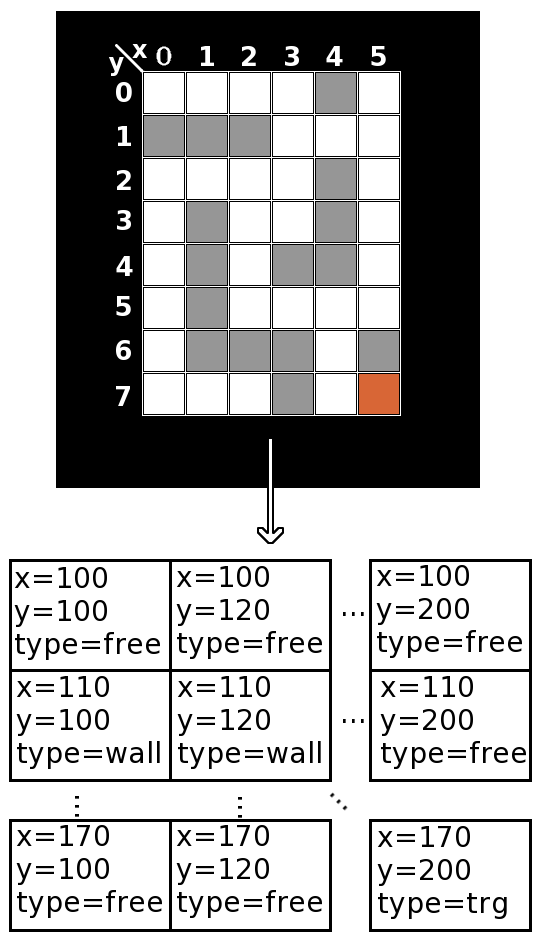
\includegraphics[width=4.5cm]{./img/MazeKheperaData.png}
        \captionof{figure}[Example of min and max values]{%
        Example of min and max values -- \\
        In this example, we have: \\
        $x_{min} = 100$ \\
        $y_{min} = 100$ \\
        $\tilde{x}_{max} = 170 $ \\
        $\tilde{y}_{max} = 200 $ \\
        $x_{max} = 180 $ \\
        $y_{max} = 220 $ \\
        $x_{extend} = 8 $ \\
        $y_{extend} = 6 $
        }
        \label{fig:mkd:struct}
    }

The maze is saved in a grid before writing it in a file. We could 
save the blocks directly from the list to the file without making a 
grid, but this way we might not be able to save it serially 
from the list to the file. The objects might not be in the order needed
to print them in the file.
As it is right now, the objects are already in-order when they are 
send from the MazeDetector, so we could save it directly in a file 
without saving it in a grid. But by doing this, an in-order list of 
objects would be a prerequisite. By saving the blocks in a grid to be 
sure that we have the blocks in-order, we could, for whatever 
reason, send objects in random order and it would work as well. 
\\
\\
We could have transferred the data directly to MazeData without saving 
it in a maze definition file. We could have inherited from MazeData 
to do so. But we would need to modify some part of MazeData as they 
are not private but protected. Also and most of all, 
MazeReward and MazeGraphic rely 
on the maze definition file to build their maze definition. They could 
use the new MazeKheperaData, but it is better if we can avoid 
modifying more modules.
\\
\\
Whenever someone wants to modify the mapping of the block information 
(x=x,y=y,size=color index) or add new types for blocks (trap for example), 
the lines to modify are in the loop of 
the save\_maze() function. See the improvements subsection 
\ref{sec:cgd:improvements} of colored 
grid detector for more information on this.

\subsection{How to use}
\label{sec:mkd:howto}

The maze detector must be on. You need to pass the corresponding 
configuration file for the detector to the class and give a file name 
to save the maze in the constructor; MazeKheperaData(tapir\_conf\_file,
filename). 

You can then use the functions get\_RX() and get\_RY() to get the (X\_i,Y\_i) 
values of the image from the ($x_g$, $y_g$) coordinates of the grid. Also, 
you can use get\_centered\_RX() and get\_centered\_RY() to get the 
($x_i$, $y_i$) 
in the center of the block in the image from the ($x_g$, $y_g$) coordinates 
of the grid.
